\chapter{Evaluation}
\label{sec:evaluation}

% Zu jeder Arbeit in unserem Bereich gehört eine Leistungsbewertung. Aus
% diesem Kapitel sollte hervorgehen, welche Methoden angewandt worden,
% die Leistungsfähigkeit zu bewerten und welche Ergebnisse dabei erzielt
% wurden. Wichtig ist es, dem Leser nicht nur ein paar Zahlen
% hinzustellen, sondern auch eine Diskussion der Ergebnisse
% vorzunehmen. Es wird empfohlen zunächst die eigenen Erwartungen
% bezüglich der Ergebnisse zu erläutern und anschließend eventuell
% festgestellte Abweichungen zu erklären.


\begin{itemize}

\item What should be evaluated
  \begin{itemize}
  \item Performance evaluation
  \item Design evaluation (lines of code, reusability)
  \item Flexibility evaluation
  \end{itemize}

\item Objective is not to implement efficient simulation, but
  it should demonstrate the developed system in its functionality
  and in comparison with MPI.

\item Own expectations
  \begin{itemize}
  \item Not much overhead compared to MPI implementation
  \item Expect the usual communication behavior
  \item less communication over network means less delay
  \item the more local calculation the more performance
  \item The software should perform as fast as the
    underlying adapter
  \end{itemize}

\item Measurements
  \begin{itemize}
  \item Configuration of the developed system (CAL, GRAPH, GVON)
  \item simulations steps per minute
  \item Idea Axel: Delay calculation of some cells
    Remap peers such that execution time of all peers
    will be the same again.
  \item Varying cluster node konfigurations
    \begin{itemize}
    \item Use different amounts of nodes
    \item Use different cluster queues
    \item Use different mapping methods
    \item Evaluate the methods and whether they
      behave like expected.
    \end{itemize}
  \end{itemize}

\item The benchmark system for evaluation was HPC system of the
  Helmholz Zentrum Dresden Rossendorf \cite{ref:hzdr_cluster}.  A part
  of the system is the hypnos linux cluster (Ubuntu 12.04.4 LTS)
  constisting of two headnodes and more than 150 compute nodes. The
  node hardware ranges from AMD Italy Opterons with two core to AMD
  Interalagos Opterons with 16 cores. Furthermore, some nodes are
  equipped with Intel Xeon CPUs with 4 cores.

  The so called laser nodes combine 4 AMD Interlagos Opterons by 4
  sockets on a single mainboard resulting in 64 CPUs per node.  The
  Interlagos Opterons 6276 are two Valencia chips on a single die,
  whereby 2 core share a 64 KByte L1 Cache and a 2 MByte L2
  Cache. Laser nodes are interconnected by an Infiniband
  network. These nodes are interesting for benchmarking, since even
  one laser node has a very complex stucture

  \sitem{MPI version 1.6.3}
  \sitem{GCC 4.8.2 and application compiled with O3}


  \begin{itemize}
  \item hypnos with Linux Ubuntu 12.04.4 LTS
  \item Laser queue
    \begin{itemize}
    \item 4 sockets x 16 core AMD Opteron 6267 Interlagos = 64 core 
    \item AMD Opteron 6267 is Multi-Chip Modul (2 Valencia CPU)
    \item Nodes are connected by Infiniband
    \item 256 GB main memory
    \end{itemize}
  \item k20 queue
    \begin{itemize}
    \item 2 sockets x 4 core Xeon 2.4 GHz
    \item Nodes are connected by Infiniband
    \end{itemize}
  \item Network: Infiniband and Ethernet
  \item Communication library
  \end{itemize}
\end{itemize}

%%%%%%%%%%%%%%%%%%%%%%%%%%%%%%%%%%%%%%%%%%%%%%%%%%%%%%%%%%%%%%%%%%%%%%%%%%%%%%%%
%                                                                              %
% SYNTHETIC POINT TO POINT BENCHMARK                                           %
%                                                                              %
%%%%%%%%%%%%%%%%%%%%%%%%%%%%%%%%%%%%%%%%%%%%%%%%%%%%%%%%%%%%%%%%%%%%%%%%%%%%%%%%
\subsection{Synthetic Point to Point Benchmark}

This synthetic benchmark compares the runtime of fundamental point to
point communication operations of MPI with CAL and GVON. It should
determine the runtime overhead of CAL and GVON in respect to a plain
usage of MPI. The source code for this benchmark is free from any
application logic. Since this benchmark does not represent a real
world application, it does only contain communication operations of
the particular abstraction layer.

Two peers are exchanging data. Whereby, one peer is the sender and the
other is the receiver. The time is measured for an experiment of
sending and receiving of n messages with m elements. Such an operation
will be called send/recv operation. Every experiment is executed 100
times and then averaged to reduce variations in runtime. An experiment
configuration has the following parameters:

\begin{itemize}
  \item Number of consecutive send and receive operations
  \item Number of send/receive elements
  \item Communicating with and without network
  \item Selection of compute nodes kepler or laser
\end{itemize}

For the following experiments in this benchmark, a single parameter is
variated while the others stay on a fixed values. This should evaluate
the impact of this parameter in respect to the MPI implementation.

\subsubsection*{Increase number of consecutive send and receive operations}
This experiment increases the number of consecutive send/recv
operations from 1 to 10e3 by a stepsize of 10. Thereby, the amount of
sending and receiving data is set fixed to 4 Byte (integer).  The
runtime for these consecutive send/recv operations is measured and
then averaged to obtain the runtime for a single operation.
Figure \ref{fig:nsend_kepler} shows the averaged runtime on a single
kepler node.


\begin{figure}[H]
  \label{fig:nsend_kepler}
  \begin{minipage}[t]{0.5\textwidth} 
    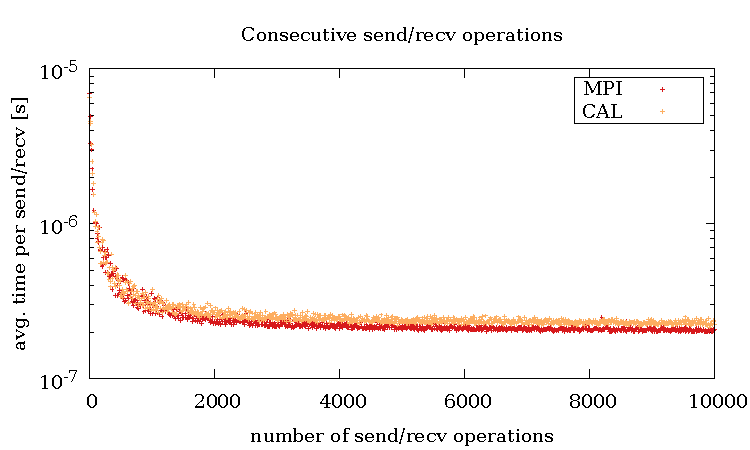
\includegraphics[width=\textwidth]{plots/50_nsend_cal_kepler}
    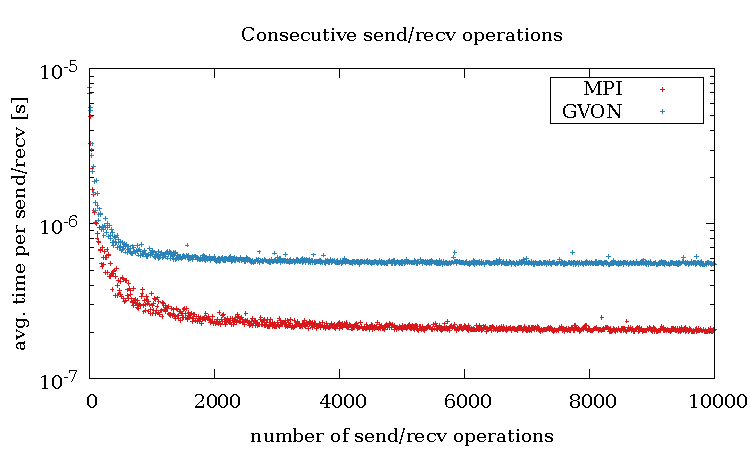
\includegraphics[width=\textwidth]{plots/50_nsend_gvon_kepler}
    \end{minipage}
  \begin{minipage}[t]{0.5\textwidth}
    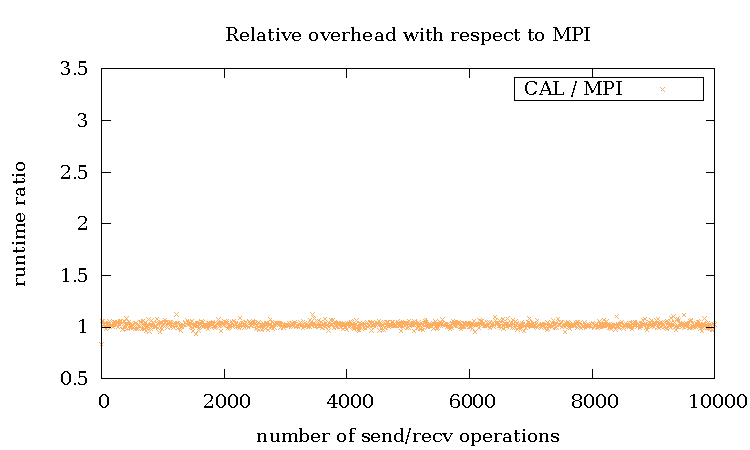
\includegraphics[width=\textwidth]{plots/50_nsend_overhead_cal}
    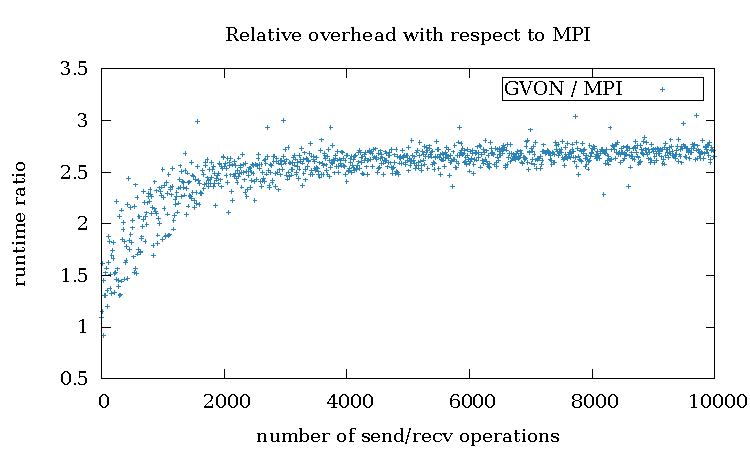
\includegraphics[width=\textwidth]{plots/50_nsend_overhead_gvon}
  \end{minipage}

\end{figure}

\sitem{CAL has 10\% constant overhead in respect to MPI}
\sitem{CAL has 177\% constant overhead in respect to MPI}

\todo{Compare MPI, CAL, GVON}
\todo{Compare kepler and laser nodes}
\todo{Compare with and without network}


The GVON has a big constant overhead per send/recv operation in
respect to MPI. This overhead is explainable: since the
communication topology of the GVON is described by a graph including 2
nodes connected by a directed edge, the constantly lookup in the graph
adds constant overhead to each send/recv operation.  Instead, CAL and
MPI are sending and receiving from fixed peer addresses. The graph is
not changing during the experiment. Thus, it is sufficient to perform
the graph lookup only once. Figure \ref{fig:nsend_one_lookup_kepler}
shows the same experiment, but the GVON performs only one lookup.

\begin{figure}[H]
  \caption{ }
  \label{fig:nsend_kepler}
  \begin{minipage}[t]{0.5\textwidth} 
    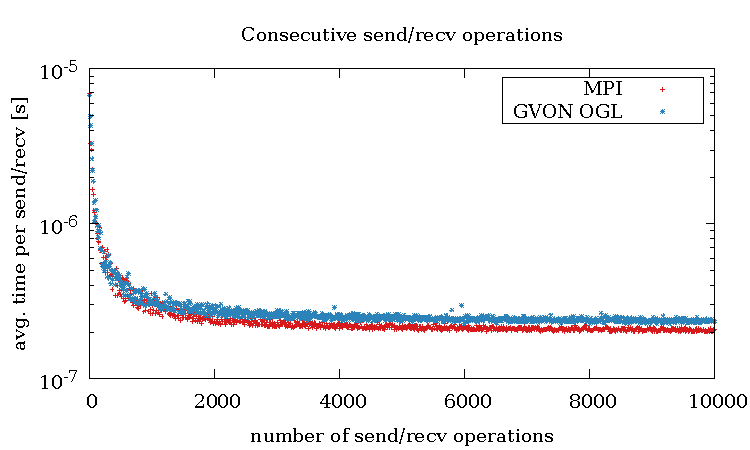
\includegraphics[width=\textwidth]{plots/50_nsend_one_lookup_kepler}
  \end{minipage}
  \begin{minipage}[t]{0.5\textwidth}
    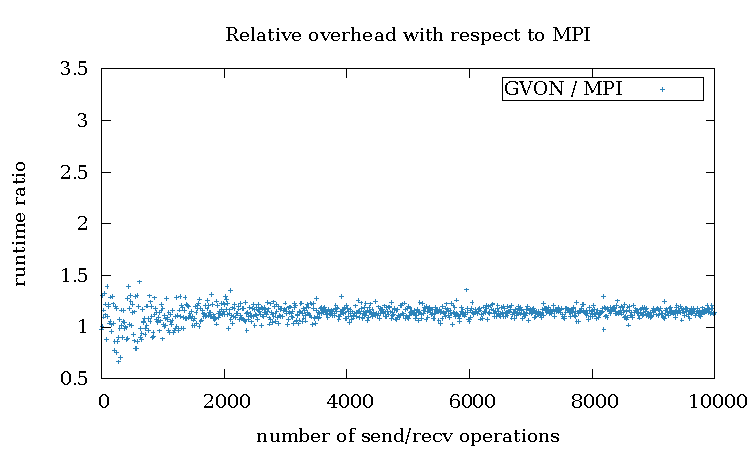
\includegraphics[width=\textwidth]{plots/50_nsend_one_lookup_overhead_gvon_kepler}
  \end{minipage}
\end{figure}

The one lookup version of the experiment reduces the GVON overhead
to same level like the CAL. It shows that the graph implementation
need to be optimized with regard to lookup of incoming and
outgoing edges.

\subsubsection*{Increase number of elements per send and receive operations}
This experiment increases the number of elements per send and receive
operation from 1 to 10e3 by a stepsize of 10. A single experiment
obtains the average runtime over 1000 send and receive operations.
Figure \ref{fig:nsize_laser} shows the averaged runtime to send and
receive a single element on a laser node.

\begin{figure}[H]
  \centering 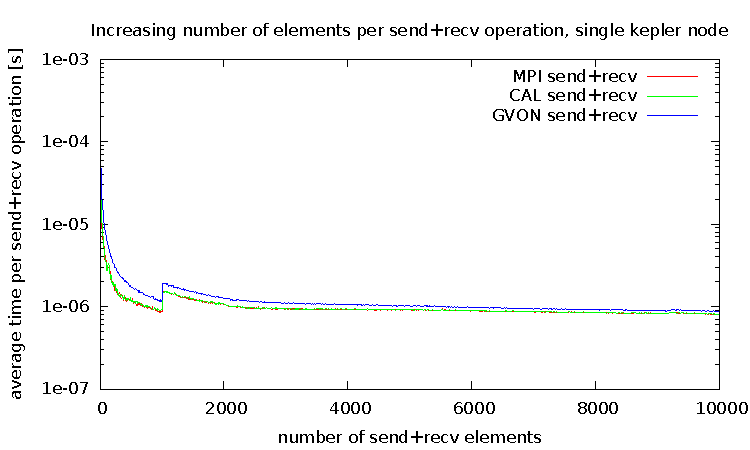
\includegraphics[width=\textwidth]{plots/50_nsize_kepler}
  \caption{ }
  \label{fig:nsize_laser}
\end{figure}

\sitem{Decreasing overhead when number of elements increases}
\sitem{Since overhead is constant}

\sitem{Compare kepler and laser nodes}
\sitem{Compare MPI, CAL, GVON}
\sitem{Compare with and without network}
\sitem{Examine differences between data types (there should be no difference)}

%%%%%%%%%%%%%%%%%%%%%%%%%%%%%%%%%%%%%%%%%%%%%%%%%%%%%%%%%%%%%%%%%%%%%%%%%%%%%%%%
%                                                                              %
% SYNTHETIC COLLECTIVE BENCHMARK                                               %
%                                                                              %
%%%%%%%%%%%%%%%%%%%%%%%%%%%%%%%%%%%%%%%%%%%%%%%%%%%%%%%%%%%%%%%%%%%%%%%%%%%%%%%%
\subsection{Synthetic Collective Benchmark}
\begin{itemize}
\item Synthetic Send/Recv Tests
\item Synthetic Collective Tests
  \begin{itemize}
  \item GVON only implements gather and reduce
  \item N collective operations
  \item average runtime of one collective operation
  \item Increase amount of data to send
  \item Varying data types
  \item Compare MPI, CAL, GVON
  \end{itemize}

\end{itemize}

%%%%%%%%%%%%%%%%%%%%%%%%%%%%%%%%%%%%%%%%%%%%%%%%%%%%%%%%%%%%%%%%%%%%%%%%%%%%%%%%
%                                                                              %
% GAME OF LIFE BENCHMARK                                                       %
%                                                                              %
%%%%%%%%%%%%%%%%%%%%%%%%%%%%%%%%%%%%%%%%%%%%%%%%%%%%%%%%%%%%%%%%%%%%%%%%%%%%%%%%
\subsection{Game of Life Benchmark}
The GoL benchmark compares the presented GoL implementation with an
equivalent MPI implementation. Equivalent refers to the same set of
rules, the same amount of communication operations and the same
functions are used to update the cell states.


\begin{itemize}
\item Simple Game of Life
  \begin{itemize}
  \item Single cell per vertex or MPI process
  \item Peer hosts several vertices
  \item Common GoL rules
  \item Next neighbor communication in a 2D Grid with diagonal connections
  \item Just a simple example
  \item But cells can be even more complex
  \end{itemize}
\end{itemize}

%%%%%%%%%%%%%%%%%%%%%%%%%%%%%%%%%%%%%%%%%%%%%%%%%%%%%%%%%%%%%%%%%%%%%%%%%%%%%%%%
%                                                                              %
% N BODY BENCHMARK                                                             %
%                                                                              %
%%%%%%%%%%%%%%%%%%%%%%%%%%%%%%%%%%%%%%%%%%%%%%%%%%%%%%%%%%%%%%%%%%%%%%%%%%%%%%%%
\subsection{N Body Benchmark}
This benchmark simulates the implemented n body simulation for 1000
timesteps with increasing number of bodies. It is compared a
simulation implemented with MPI to one implemented with the GVON. In
contrast to the synthetic benchmark, calculations have to be performed
inbetween communication operations. Thus, the communication operations
do not provide the main runtime. Figure \ref{fig:nbody_laser} shows
the averaged runtime of a timestep with increasing number of bodies.

\begin{figure}[H]
  \centering 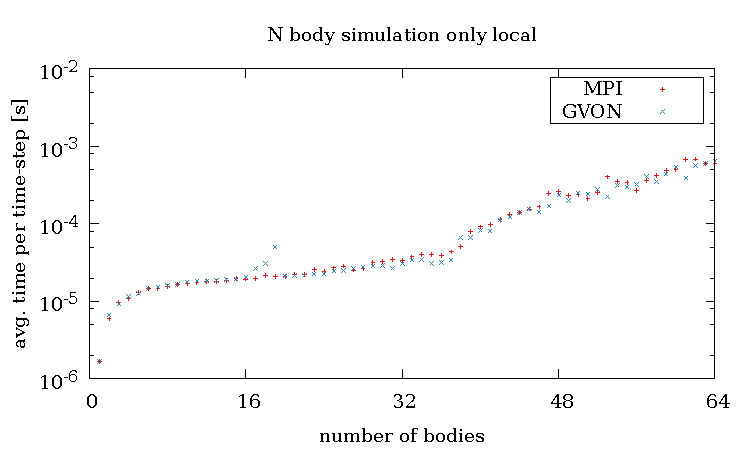
\includegraphics[width=\textwidth]{plots/50_nbody_laser}
  \caption{ }
  \label{fig:nbody_laser}
\end{figure}

The average runtime of a timestep raises quadratically with the number
of bodies. Also the variance increases quadratically. Thus, the runtime
of the timesteps variates strongly.

\sitem{Still no explaination for strong variance}


\begin{itemize}
  \item Simple N-Body
    \begin{itemize}
    \item 1 to 256 Bodies
    \item runs on laser machine (64 CPUs)
    \item run of 1000 timesteps
    \item max 4 bodies per CPU
    \item Compare with and without network
    \item Compare MPI with GVON
    \item Compare different amount of CPUs
    \end{itemize}
\end{itemize}


%%%%%%%%%%%%%%%%%%%%%%%%%%%%%%%%%%%%%%%%%%%%%%%%%%%%%%%%%%%%%%%%%%%%%%%%%%%%%%%%
%                                                                              %
% CONCLUSION                                                                   %
%                                                                              %
%%%%%%%%%%%%%%%%%%%%%%%%%%%%%%%%%%%%%%%%%%%%%%%%%%%%%%%%%%%%%%%%%%%%%%%%%%%%%%%%
\begin{itemize}
\item Conclusion about evaluation points. What can
  be done better, where can the system be changed.
  Give reason for behavior of the system.

\end{itemize}

\cleardoublepage

%%% Local Variables:
%%% TeX-master: "diplom"
%%% End:
